% UTF-8

% single-chapter commands
\documentclass[../main/thesis.tex]{subfiles}
\onlyinsubfile{\setcounter{chapter}{4}}  % single-chapter command
\begin{document}


\chapter{Implementierung}

\section{Entwicklungsumgebung}

Zur Umsetzung der entwickelten Algorithmen in Software wurde die Plattform Java verwendet.
Die Wahl von Java erfolgte neben der Vertrautheit des Verfassers mit dem zugehörigen \term{framework} aufgrund zu erwartender Effizienzvorteile von kompiliertem Code gegenüber Skriptsprachen wie Perl.
% einer Empfehlung der Geofabrik folgend

Java als imperative Sprache erlaubt es nicht, Algorithmen mit dem gleichen Grad an Abstraktion zu beschreiben wie zuvor in Kapitel~\ref{ch:algorithm-parts} geschehen.
Dort konnten zugunsten einer vereinfachten
% jedoch präzisen, cf. EWD656
Beschreibung praktische Erwägungen wie der Bedarf an Rechenzeit und Speicherplatz teilweise hintenanstehen.
Bei der Implementierung in Java müssen hingegen sorgfältig solche Datenstrukturen gewählt werden, die eine effiziente Ausführung erlauben, und die Algorithmen soweit nötig entsprechend angepasst werden.
Das Ergebnis wird in Abschnitt~\ref{ch:data-structures} beschrieben.

Während der Entwicklung wurde versucht, so viel existierenden Code in Form von \term{frameworks} wiederzuverwenden wie möglich.
Diese Bestrebung verursachte Probleme, wie auch später in Abschnitt~\ref{ch:impl-difficulties} geschildert wird.
Bei der Entwicklung kamen zuletzt die folgenden Plattformen und \term{frameworks} zum Einsatz:

\begin{itemize}[nosep]
	\item Darwin 15.6 / Mac OS X 10.11.6
	\item Java™ Standard Edition JDK 8 Update 152\\ \url{http://www.oracle.com/technetwork/java/javase/downloads/}
	\item Apache Ant 1.10.1 \quad \url{https://ant.apache.org/}
	\item args4j 2.33 \quad \url{http://args4j.kohsuke.org/}
	\item GeoTools 18.0 \quad \url{http://www.geotools.org/}
	\item TestNG 6.8 \quad \url{http://testng.org/}
	% http://web.archive.org/web/20121113133417/http://testng.org/testng-6.8.zip (all other releases appear to be corrupt; I'm probably doing something wrong)
	\item GDAL 2.2.2 \quad \url{http://www.gdal.org/}
\end{itemize}

Ursprünglich wurden ältere Softwareversionen verwendet.
Die nötigen Anpassungen an die hier genannten aktuellen Versionen waren gering, Kompatibilität mit den älteren Versionen ist jedoch gegenwärtig aufgrund von Änderungen in GeoTools nicht mehr gegeben.
Der Code ist dabei noch immer konform zum Syntax von Java 6. \cf{GJSB05}

Der folgende Abschnitt erläutert einige Überlegungen, die bei der Auswahl der \term{frameworks} relevant waren.



\section{Systemkonzept}

Für ein gut funktionierendes Gesamtpaket sind vor der Umsetzung von vorgegebenen Algorithmen in ausführbarem Code einige praktische Aspekte zu bedenken.

Zunächst stellt sich die Frage nach der Benutzerschnittstelle der Software.
Die gewählte Plattform Java bietet verschiedene Möglichkeiten, graphische Benutzeroberflächen (GUI) zu gestalten.
Denkbar wäre beispielsweise eine Integration in den weit verbreiteten \osm-Editor JOSM als \term{plug-in.}
Das Entwickeln und Debuggen einer GUI-Anwendung neigt jedoch dazu, zeitaufwändig zu sein.
Ohnehin würde es ein modularer Aufbau der Anwendung erlauben, zu einem späteren Zeitpunkt eine GUI zu ergänzen.
Aus diesen Gründen soll im Rahmen dieser Arbeit auf eine GUI zugunsten einer einfachen textbasierten Kommandozeilen-Schnittstelle (\term{command-line interface,} CLI) verzichtet werden.
Zum Parsen der CLI-Parameter bieten sich \term{frameworks} wie etwa args4j an.

Zur Verarbeitung beliebiger Geodaten müssen diese aus Datenspeichern eingelesen und wieder ausgegeben werden können.
Um Entwicklungszeit zu sparen, sollte hierfür nach Möglichkeit ein existierendes \term{framework} genutzt werden.
Zur Vermeidung einer zu engen Kopplung der Generalisierung an das gewählte \term{framework} ist es zu vermeiden, die Primitiven des \term{frameworks} intern weiterzubenutzen.
Stattdessen sollten eigene Datenstrukturen genutzt werden, um Modularität zu fördern.
Die dabei entstehenden Kosten in Form von Rechenzeit und Speicherverbrauch sind zu berücksichtigen.

Da die Algorithmen auf der euklidischen Ebene definiert sind (vgl. Abschnitt~\ref{ch:split-algorithm}), bietet es sich an, die Implementierung zunächst auf kartesische Koordinaten zu beschränken und zu verlangen, dass aus der \osm-Datenbank stammende Eingangsdaten nach Länge und Breite vor der Verarbeitung vom Benutzer in einem geeigneten Kartennetzentwurf abgebildet werden.
Grundsätzlich wären angesichts der hier durchzuführenden geometrischen Operationen winkeltreue Abbildungen wie etwa ein Mercator-Netz zu bevorzugen.
% Sny87, USGS PP 1395 p. 20
Aufgrund der üblicherweise geringen Abstände der Parallelen ist Winkeltreue jedoch kein strenges Kriterium.
% Wiederholung eines ähnlichen Gedanken in 4.3.1

Die in Abschnitt~\ref{ch:split-algorithm} gegebene Definition für \textproc{NaheSegmente} kann leicht mit Hilfe eines R-Baums umgesetzt werden.
Die \textproc{Hülle} ist dabei das minimal umgebende Rechteck eines Blatts im R-Baum.
Nachdem die \osm-Eingangsdaten vor der Generalisierung vollständig bekannt und somit statisch sind, bietet sich der Einsatz eines gepackten R-Baums an \cf[255-256]{RSV02}.
Ein solcher Baum wird von der JTS Topology Suite (JTS) angeboten, welche vom \term{framework} GeoTools als Implementierung des Geometriemodells verwendet wird.

GeoTools bietet außerdem Möglichkeiten zur Ein- und Ausgabe (\term{input/output,} I/O) von Geodaten in zahlreichen Formaten.
Zwar wird das native \osm-XML-Format ebensowenig unterstützt wie das neuere Protocol Buffer Binary Format (PBF).
Das verbreitete Format ESRI~Shapefile wird jedoch unterstützt.
Die Geofabrik stellt aktuelle OSM-Auszüge öffentlich als Shapefile bereit.
Alternativ lassen sich Shapefiles leicht mit gängiger Software wie etwa GDAL aus anderen Formaten erzeugen.
GDAL ermöglicht dabei auch den Zuschnitt auf ein abgegrenztes Untersuchungsgebiet, was sich für Testzwecke anbietet.

\onefigure{ht}{
	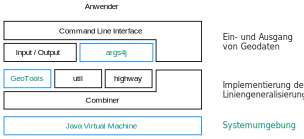
\includegraphics[width=\ScaleIfNeeded]{../chapter5/system-concept}
	\caption{Systemkonzept (schwarz: eigene Entwicklung, blau: benutztes \term{framework})}
	\label{fig:system-concept}
}

Zusammengesetzt ergibt sich aus den besprochenen Aspekten der in Abbildung~\ref{fig:system-concept} dargestellte Systemaufbau:
Dem Anwender steht eine Kommandozeilen-Schnittstelle (CLI) zur Verfügung, die ihrerseits das \term{framework} args4j zum Parsen der Parameter sowie selbst entwickelte Routinen zur Ein- und Ausgabe der Geodaten verwendet.
Die CLI steuert damit die eigentliche Liniengeneralisierung (hier als „Combiner“ bezeichnet), welche ihrerseits neben dem \term{framework} GeoTools noch einige selbst entwickelte Hilfsmodule verwendet, die nicht vom Combiner abhängig sind und deshalb als separates Softwarepaket dargestellt werden (mit „util“ bezeichnet).

% Noch mal Modularisierung; java Packages erwähnen/erklären? -> eher nein



\section{Datenstrukturen}
\label{ch:data-structures}

% Einleitung/Überleitung:
% - im Folgenden wird insbesondere der Combiner näher beschrieben
% - es werden nur wesentliche Aspekte behandelt und im Übrigen auf API-Doku und Source Code verwiesen
% - übergeordnete Frage: warum _so_ und nicht anders?

% ===========================
% Erstens: Warum eigene Elementare, warum nicht die von GeoTools nehmen?
% Einige Algorithmen, zB. SPLITTEN und ANALYSE, ordnen den Segmenten zusätzliche Daten zu (wurzel/closeParallels). Dies unterstützt JTS zwar in Form von "user data objects". Weil jedoch die Arbeit damit eher umständlich ist, wäre dies nur sinnvoll, wenn die Nutzung der JTS-Geodatenstrukturen andere Vorteile bietet.
% Dies ist jedoch nicht der Fall. Im Gegenteil passen die JTS-Datenstrukturen nicht 100%ig auf meine Algorithmen: Algorithmen beschränken sich zu einem großen Teil auf Segmente aus exakt zwei Nodes, während JTS von längeren Linienzügen ausgeht.
% Die Algorithmen machen sich außerdem zunutze, dass Segmente sich direkt als Vektoren interpretieren lassen. Routinen zur Vektor-Mathe bietet JTS zwar grundsätzlich an, jedoch sind wichtige Teile davon nicht spezifiziert und damit nicht verlässlich verwendbar (Beispiel: math.Vector2D: angle, vgl. Algorithmus ANALYSE)
% Abgesehen vom Spatial Index scheinen auch JTS-Manipulationen mir recht wenig zu helfen.
% Direktes Verwenden der bereitgestellten JTS-Datenstrukutren deshalb eher nicht sinnvoll.
% => eigene Klassen!
% evtl. lassen sich, wie in Nr. 8 im "JTS Topology Suite Developer’s Guide" 1.4 beschrieben, die Interfaces (z. B. CoordinateSequence) implementieren, damit die eigenen Klassen von Dritten mit JTS direkt genutzt werden können. Für dieses Projekt hat dies allerdings keinen besonderen Nutzen.

% ===========================
% Zweitens: ER-Modell präsentieren
% Design-Entscheidungen darin anhand von Kap. 4 begründen
%   https://de.wikipedia.org/wiki/Assoziation_(UML)#Aggregation_und_Komposition

% Für 4.3.1 ergibt sich folgendes Datenmodell:
% [Dataset]1 <>-- 0…n[Line]1 <>-- 1…n[Segment]1…n <>-- 2[Node]
% Die Segmente sind wie in 4.3.1 beschrieben zunächst nicht in den Eingangsdaten vorhanden, sie herzustellen ist jedoch eher trivial (SEGMENTIERUNG)
% Die hier (in Abb. "Datenmodell") gezeigten Datenstrukturen wurden als Interfaces (formale Schnittstellendefinition) umgesetzt, um ihre eventuelle Wiederverwendung zu erleichtern. [cf. GHJV p18]
% Bei der Implementierung entstand folgende Klassenstruktur:
% [Klassenstruktur "Splitten"]

% Die Anzahl der jeweils das Interface implementierenden Klassen ist in diesem Projekt klein, so dass es sich anbietet, die jeweiligen Gemeinsamkeiten in abstrakten Klassen zusammenzufassen, um Redundanzen zu vermeiden. Diese Klassen gehören daher zu den umfangreicheren im Projekt.
% Wie in 4.3.1 erläutert, existiert derjenige node, an dem Segmente beim SPLITTEN zerteilt werden, nicht in den Eingangsdaten. Dementsprechend wird unterschieden zwischen SourceNode (aus OSM kommend) und NonexistentNode (entstehen beim SPLITTEN). Beide implementieren jedoch die gemeinsame Schnittstelle für den Typ Node. Zu den Gemeinsamkeiten für Nodes gehören in erster Linie deren Koordinaten, die folglich von der Klasse AbstractNode verwaltet und von den beiden konkreten Implementierungen geerbt werden.
% In gleicher Weise fasst AbstractSegment Gemeinsamkeiten solcher Segmente, die direkt aus den Eingangsdaten stammen (SourceSegment), und solcher Segmente, die erst durch SPLITTEN eines Segments entstehen (Fragment), zusammen. In Abschnitt 4.3 wurden solche Segmente zur Vereinfachung einander gleichgestellt. Für derartige Fälle schlagen Gamma et al. den Einsatz des Composite-Patterns vor: „Use the Composite pattern when […] you want clients to be able to ignore the difference between compositions of objects and individual objects. Clients will treat all objects in the composite structure uniformly.“ [GHJV p164]

% TODO:
% - Begründen, warum Bridge notwendig wäre und warum sie nicht gebaut wurde!
% - Beim SPLITTEN passiert ... was?
% In diesem speziellen Fall wird die Struktur der Komposition nur durch SPLITTEN verändert. Dabei wird genau ein Segment durch zwei andere ersetzt, die gemeinsam das ersetzte Segment repräsentieren.
% Dies entspricht zwar dem Composite-Leaf–Modell des Composite-Patterns, aber weil diese Unterscheidung orthogonal zur Unterscheidung in SourceSegment/Fragment ist, 

% TODO:
% soll tatsächliches Objektmodell für Fragmente gezeigt werden oder verwirrt das nur?

% TODO:
% Die Unterschiede zwischen SourceSegment und Fragment sind zunächst klein
% Hier sind zunächst nur NAHESEGMENTE implementiert.
% Envelope/closeSegments in SOurceSegment sollte laut 4.3.1 auf jedes Segment anwendbar sein, ist tatsähchlich nur auf SourceSeg. implelentiert. Macht aber nix, denn laut 4.3.1 dient NaheSegmente ausdrücklich nur der Effizienzsteigerung, und dem läuft zuwider, dass der R-Ttree nicht verändert werden sollte. Die Korrektheit wird dann laut 4.3.1 über die erneute Abstandsprüfung in der Analyse gesichert.

% TODO:
% Vector erwähnen!

% (weitere Besonderheiten der Konkreten ggü. Abstract*?)
%- SourceNode enthält neben der ID nur Pointers zu den Segmenten etc. für die Korralation
%- SourceSegment außerdem nur L+R sowie analyseLineParts

% ===========================
% Analyse und Punktezuordnung

% Die Analyse (4.3.2) ändert das Datenmodell nur unwesentlich: SourceSegment bekommt L+R
% Unterschied in Implementierung: es wird eine Liste gepflegt. TODO: Testen: Unterscheidet sich der Output, wenn die Liste auf das jeweils nächste Element reduziert wird?

% TODO: Visitor

% Für 4.3.3 ergibt sich folgendes Datenmodell/Klassenstruktur:
% [CorrelationGraph]1 <>-- 1…n[CorrelationEdge]0…n <>-- 2[Node]
% zusätzlich bekommt SourceNode wenigstens schon mal einige der Pointers, wenn nicht schon alle

% ===========================
% Liniengeneralisierung 4.3.4

% Datenmodell/Klassenstruktur:
% [GeneralisedLines]1 <>-- 0…n[ResultLine (Section/GeneralisedSection)]0…n <>-- 2…n[Node]

% TODO: 4.3.4 spricht hier von Segmenten, die aneinandergehangen werden. Eventuell passiert das hier mit Nodes? Nochmal prüfen! Macht aber eigentlich keinen großen Unterschied.
% ...

% TODO: Big Renaming #3 (de.thaw.thesis.comb)
%OsmDataset			Dataset √
%   special uses (to be reconsidered):
%   - Output for debugging
%   - Corr.Graph to get all segments
%   - Gen.Lines to get all segments and to get midPoints
%   - AbstractSegment for debugging (parallelFragment sink etc.)
%OsmTags			Attributes / io.OsmTags ******
%OsmWay				io.OsmHighway
%   new interface:	ResultLine
% erhebliche Redundanzen in Section/GeneralisedSection - was machen wir damit? AbstractSection?

% code currently contains a lot of special-cases for debugging as well as testing:
% - CombinerMain: iterations / combineLines2
% - MyAnalyser: evaluateTags
% - pervasive debug output needs to be overhauled; perhaps as a common sink/listener



% ===========================
% Drittens: Zusammenfassung und ggf. Datenfluss/Interaktionswege
% (weichen im imperativen Code teils deutlich von funktional formulierten Algorithmen ab)



% ===========================
% Anhänge:
% - komplettes ER-Modell
% - komplette Klassenstruktur
% - evtl. Auflösung der in Kap. 4 definierten Algorithmen zu ihren Implementeriungsorten:
% SEGMENTIERUNG: OsmWay.segmentation
% SPLITTEN: SplitQueueIterator=S' (in Combiner.splitSegments), AbstractLine.splitCloseParallels()=für alle n/t, T enthält schon eine Parallitätsprüfung (warum? - in splitTargets/closeParallels)
% NAHESEGMENTE: Combiner.regionaliseSegments (arbeitet auf SourceSegments, also auf S statt S' und wurzel(s) statt s, weil so die Schnittmengenprüfung nicht wiederholt ausgeführt werden muss und damit ein Spatial Index erleichtert/ermöglicht wird)
% HÜLLE: SourceSegment.envelope
% FUSSPUNKT: AbstractSegment.findPerpendicularFoot
% ANALYSE: AbstractSegment.analyse
% PARALLEL: SourceSegment.closeParallels / MyAnalyser
% DISTANZ: MyAnalyser.evaluate
% NODESZUORDNEN: CorrelationGraph.createGraph
% ZUSAMMENFASSEN: ... (GeneralisedLines/GeneralisedSection)



\begin{itemize}
	\item konzeptueller Überblick der entwickelten Software in dem Umfang, der für den Leser dieser Arbeit zum Verständnis notwendig ist
	\begin{itemize}
		\item z. B. Klassenstrukturen
		\item z. B. Interaktionswege
	\end{itemize}
	\item Erläuterung wichtiger Designentscheidungen
	\item Unterschiede zu den entworfenen Algorithmen
	\item Bezug zu Kapitel 4 herstellen
\end{itemize}



\section{Schwierigkeiten bei der Umsetzung}
\label{ch:impl-difficulties}

% - I/O erfolgt nicht in OSM-Format
% - shapefile-Probleme: shp support wurde in Geotools neu implementiert; ob dies die Probleme löst, wurde nicht getestet <http://web.archive.org/web/20130926213903/http://docs.codehaus.org/display/GEOTOOLS/Migrate+shapefile+to+shapefile-ng>
% - I/O-Probleme
% - Debug-Output
% - strictly-typed language vielleicht einfach keine so besonders gute Idee zum Prototyping

% TODO: commit log, Notizen und alte Screenshots/Testdaten aufarbeiten
% hier NICHT Probleme mit dem Generalisierungsergebnis oder der Korrektheit der Algorithmen besprechen (gehört zu 6)



\begin{itemize}
	\item interessante konkrete Schwierigkeiten oder Erfolge bei der Implementierung aufzeigen
\end{itemize}



% single-chapter commands
%\onlyinsubfile{\listoffigures}
%\onlyinsubfile{\listoftables}
%\onlyinsubfile{% global bibliography settings

\nocite{*}  % include works in bibliography that aren't cited anywhere in the document (for debugging)

\setbibpreamble{Die Literaturangaben sind alphabetisch nach den Nachnamen der Autoren sortiert. Bei mehreren Autoren wird nach dem ersten Autor sortiert.\par\bigskip\bigskip}

\bibliography{../references-papers,../references-manual}
%\bibliography{../references-manual}
}
\end{document}
